\section{Optimal Control of Pitch/Travel with Feedback (LQ)}\label{sec:prob3}
\label{text:problem3}

\subsection{Discrete-time LQR}
\label{text:LQR}

To eliminate the discrepency between the optimal and measured travel trajectory observed in figure \ref{fig:opt_openloop}, we augment the optimal input for every time step with a state feedback term weighted by a suitable gain matrix $K$:
\begin{equation*}
u_k = u_k^* - K (x_k - x_k^*),
\end{equation*}

or, alternatively
\begin{equation}
\label{eq:LQ_ctrl}
\Delta u_k = - K \Delta x_k,
\end{equation}

where 
\begin{align*}
\Delta x_k &= x_k - x_k^*,\\
\Delta u_k &= u_k - u_k^*.
\end{align*}

It can be shown\footnote{Its optimality is derived in numerous books, e.g. \cite{Kwakernaak1972}.} that the controller \eqref{eq:LQ_ctrl} is the optimal solution minimizing the quadratic objective function

\begin{equation*}
	J = \sum_{i=0}^{\infty} \Delta x_{i+1}^\top \tilde{Q} \Delta x_{i+1} + \Delta u_i^\top \tilde{R} \Delta u_i, \quad \tilde{Q} \ge 0,\ \tilde{R} > 0,
\end{equation*}

subject to the system dynamics \eqref{eq:dmodel}, where
\begin{equation}
\label{eq:LQ_gain}
	K = (R + B^\top P B)^{-1} B^\top P A,
\end{equation}

and $P$ is the unique positive definite solution to the discrete time algebraic Riccati equation. \eqref{eq:LQ_gain} is used as the state feedback gain in \eqref{eq:LQ_ctrl}, and the resulting Linear-quadratic regulator is implemented, with weigthing matrices $\tilde{Q}$ and $\tilde{R}$ chosen to penalize deviations in states and input for satisfactory results.

\subsection{Results and discussion}

The state penalty matrix $\tilde{Q}$ and input penalty $\tilde{R}$
\begin{equation*}
\tilde{Q} = \begin{bmatrix}4&0&0&0\\0&2&0&0\\0&0&0&0\\0&0&0&0\end{bmatrix}, \quad \tilde{R} = 0.1.
\end{equation*}
are chosen with travel accuracy in mind. Deviation in travel as well as travel rate is penalized fairly hard. Input deviation is necessary for corrections in travel and travel rate, and a low penalty is therefore chosen.

Using MATLAB's \texttt{dlqr} we obtain the LQ state feedback gain $K$. Using the optimal input sequence $u^*$ and state trajectory $x^*$ obtained from solving \eqref{eq:QP_travel} the controller is applied with results shown in figure \ref{fig:lqr}.

\begin{figure}[h]
	\centering
		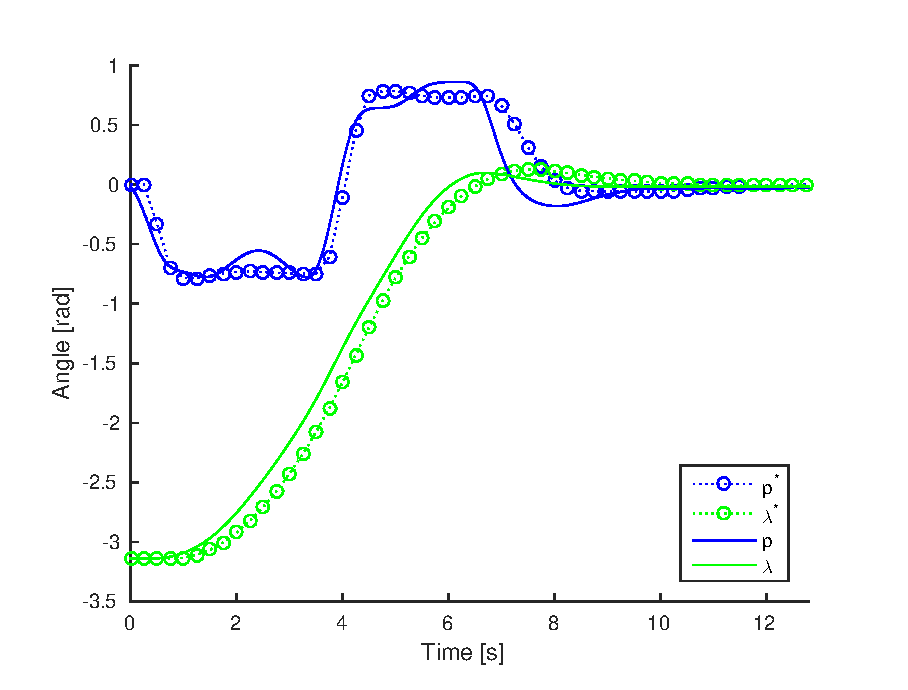
\includegraphics[width=0.85\textwidth]{figures/3/closedloop.eps}
	\caption{Optimal pitch and travel trajectories compared with measured trajectories with optimal input sequence applied in an LQR closed loop.}
	\label{fig:lqr}
\end{figure}


The measured trajectories are similar to the ones without feedback, shown in figure \ref{fig:opt_openloop}, except for the removal of travel drift over time. The travel rate model is clearly not perfect as the measured trajectory seemingly wants to deviate from the optimal path, but the discrepancies are small and the state feedback controller deals with them nicely.


\subsubsection{MPC discussion}

An alternative approach to optimal trajectories with state feedback would be to use an MPC controller. An MPC controller simply computes the optimal trajectory from the current state to the target state given a finite window of time. Only the first input of the resulting optimal input sequence is used. This is then repeated at the next iteration\footnote{Description based on \cite{Foss2014}.}. Solving an optimization problem at each time iteration is clearly computationally expensive, and even QP problems of this relatively small size would force the iteration period to increase substantially. An MPC controller with a time step on the order of several seconds is unlikely to yield better performance than a predetermined trajectory with short time steps combined with state feedback control, due to the fast dynamics of our system. Deviation from optimal trajectory is also likely to be caused by either an incomplete model or unmodeled external disturbances, and an MPC controller will not withstand either very well. 








